\section{问题三：基于库存机会成本的在线推荐策略}\label{sec:policy}

\subsection{设计思路：从离线模型到在线评分}
在线决策的难点在于当期推荐与未来库存之间的权衡。设第 $t$ 期顾客类型为 $i$、库存为 $c$，若已知第 $t+1$ 期起的最优价值函数 $V_{t+1}(\cdot)$，推荐集合 $S$ 的期望总价值为
\begin{equation}
\sum_{j\in S}p_{ij}\bigl[r_j+V_{t+1}(c-e_j)\bigr]+\Bigl(1-\sum_{j\in S}p_{ij}\Bigr)V_{t+1}(c)
=V_{t+1}(c)+\sum_{j\in S}p_{ij}\bigl[r_j-\theta_j\bigr],
\label{eq:lookahead}
\end{equation}
其中 $\theta_j=V_{t+1}(c)-V_{t+1}(c-e_j)$ 是一件商品 $j$ 的机会成本。式\eqref{eq:lookahead}的最优集合由评分 $p_{ij}(r_j-\theta_j)$ 最高、且评分非负的至多 $K$ 件有货商品组成。动态规划可以给出精确的 $\theta_j$，但其状态数为 $\prod_j(C_j+1)$，商品数增加时无法求解。

问题二的离线模型提供了一个可扩展的近似。第 $t$ 期之后还有 $\tau=T-t$ 位顾客，预计各类型人数为 $\tau\lambda$，用剩余销售期的流体线性规划 $F(\tau\lambda,c)$ 近似 $V_{t+1}(c)$，机会成本有两种计算方式：
\begin{align}
\text{对偶价格：}\quad &\theta_j=\beta_j(\tau\lambda,c),\ \text{即 }F(\tau\lambda,c)\text{ 中库存约束 }j\text{ 的对偶变量}; \label{eq:theta_dual}\\
\text{有限差分：}\quad &\theta_j=\Delta_j(\tau\lambda,c)=F(\tau\lambda,c)-F(\tau\lambda,c-e_j). \label{eq:theta_fd}
\end{align}
相应得到两种策略：\LPDual{} 每期求解一个线性规划并读取对偶价格；\LPFD{} 每期求解至多 $n+1$ 个线性规划，按式\eqref{eq:lookahead}做精确的一步前瞻。二者都在每期以最新库存重新求解离线模型，属于收益管理中的投标价格（bid-price）控制与滚动重优化\cite{talluri98,jasin,bumpensanti}。库存感知贪心 \Greedy{} 对应 $\theta=0$，即完全忽略未来。第\ref{sec:exp}节的精确评价表明，\LPDual{} 在五份数据上的期望遗憾低于 \LPFD{} 与 \Greedy{}，本文以 \LPDual{} 作为主策略，\LPFD{} 作为对照。

\subsection{机会成本的性质}
两种机会成本之间存在确定的大小关系。

\begin{proposition}\label{prop:order}
设 $\tau\ge1$，商品 $j$ 满足 $1\le c_j\le\tau$，$\beta$ 为 $F(\tau\lambda,c)$ 的任一最优对偶解，则
\begin{equation}
0\le\beta_j\le\Delta_j\le r_j.
\label{eq:order}
\end{equation}
\end{proposition}
\begin{proof}
$\beta_j\ge0$ 来自对偶可行性。记 $\mu,\nu$ 为其余约束的最优对偶变量，在库存为 $c-e_j$ 的线性规划中，$(\beta,\mu,\nu)$ 仍然对偶可行，由弱对偶得 $F(\tau\lambda,c-e_j)\le F(\tau\lambda,c)-\beta_j$，即 $\beta_j\le\Delta_j$。另一方面，取库存为 $c$ 时的一个最优解 $y$；若商品 $j$ 的期望销量超过 $c_j-1$，按比例缩小各 $y_{ij}$，使其期望销量降为 $c_j-1$。销量至多减少一件，收入至多减少 $r_j$，其余约束仍然满足，故 $F(\tau\lambda,c-e_j)\ge F(\tau\lambda,c)-r_j$，即 $\Delta_j\le r_j$。
\end{proof}

由于每期至多售出一件，$c_j>\tau$ 时商品 $j$ 在剩余期内不会售罄，可以把库存截断为 $\min\{c_j,\tau\}$ 后再求解，此时 $\Delta_j=0$。命题\ref{prop:order}说明，三种策略对稀缺商品的保守程度依次为 $\Greedy<\LPDual\le\LPFD$。$F(\tau\lambda,\cdot)$ 是分段线性凹函数，$\beta_j$ 是当前库存处的局部斜率，$\Delta_j$ 是向左一个单位区间上的平均斜率。在斜率发生跳变的位置附近，有限差分会提前计入下一段更高的边际价值。

\subsection{算法}
算法\ref{alg:dual}给出主策略 \LPDual{} 的完整步骤。离线模型\eqref{eq:lp}只在开始时建立一次，此后每期只修改约束右端项与变量上界，可以利用上一期的单纯形基热启动。

\setcounter{algorithm}{1}% the assignment's Algorithm 1 keeps its number
\begin{algorithm}[htbp]
\caption{\LPDual{}：基于线性规划对偶价格的在线 Top-$K$ 推荐}
\label{alg:dual}
\begin{algorithmic}[1]
\Require prices $r$, purchase probabilities $P$, arrival rates $\lambda$, inventory $C$, slots $K$, horizon $T$; customer types $i_1,\ldots,i_T$ revealed one at a time
\Ensure recommendation sets $S_1,\ldots,S_T$, revenue $R$, final inventory $c$
\State $c\gets C$, $R\gets 0$
\State build LP \eqref{eq:lp} once with variables $y_{ij}$ \Comment{later only RHS and bounds change}
\For{$t=1$ \textbf{to} $T$}
  \State observe $i\gets i_t$; \ $\tau\gets T-t$ \Comment{customers after the current one}
  \If{$\tau=0$}
    \State $\theta\gets 0$
  \Else
    \State $c^{\tau}_j\gets\min\{c_j,\tau\}$ for all $j$
    \State solve $F(\tau\lambda,c^{\tau})$; \ $\theta\gets\beta$ \Comment{duals of the inventory rows}
  \EndIf
  \State $E\gets\{\,j\in A(c):\ p_{ij}r_j>0,\ \ s_j:=p_{ij}(r_j-\theta_j)\ge 0\,\}$
  \State sort $E$ by $s_j$ (descending), then $p_{ij}r_j$ (descending), then $j$ (ascending)
  \State $S_t\gets$ first $\min\{K,|E|\}$ products of $E$
  \State show $S_t$ to the customer and observe the purchase $J'_t\in S_t\cup\{0\}$
  \If{$J'_t=j\neq0$}
    \State $c_j\gets c_j-1$, \ $R\gets R+r_j$
  \EndIf
\EndFor
\State \Return $(S_t)_{t=1}^{T}$, $R$, $c$
\end{algorithmic}
\end{algorithm}

\textbf{对照策略 \LPFD{}。} 把算法\ref{alg:dual}第 9 行替换为
\begin{equation*}
\textbf{for } j\in A(c)\textbf{ do }\ \theta_j\gets F(\tau\lambda,c^{\tau})-F\bigl(\tau\lambda,(c-e_j)^{\tau}\bigr)\ \textbf{end for},
\end{equation*}
其余步骤不变。

\textbf{剩余人数预测 \LPCount{}。} 若平台事先知道整个销售期各类型的总人数 $N$（例如题目给出的五份数据均为 $(50,30,20)$），可以把算法\ref{alg:dual}中的 $\tau\lambda$ 替换为剩余人数的预测
\begin{equation}
d_t=\frac{\tau}{\sum_k(N_k-n_{tk})^+}\,(N-n_t)^+,
\label{eq:countforecast}
\end{equation}
其中 $n_{tk}$ 为前 $t$ 期（含当期）已到达的类型 $k$ 顾客人数。$d_t$ 只用到已观察到的到达和总人数，不使用未来顾客的到达顺序。第\ref{sec:order}节用它衡量到达顺序信息的价值。

\textbf{评分规则的细节。} 第 11 行要求 $p_{ij}r_j>0$，从而购买概率为零的商品不会占用推荐位。评分等于零的商品仍可进入推荐列表：机会成本等于价格时，推荐该商品与空出推荐位的近似价值相同，而前者在库存最终未被占用时还能带来收入。评分相同时优先即时收益较高的商品，再按编号排序，因此策略是状态的确定性函数。比较评分前把数值舍入到 $10^{-9}$，以消除单纯形求解的浮点误差。需要指出，评分并列并非偶然：由互补松弛条件，流体最优解中被同一类顾客混合使用的推荐集合，其调整后收益必然相等。例如 $\beta^{*}=(9,0,0)$ 时，类型 1 顾客对商品 1 与商品 3 的评分都等于 $0.6$。并列规则因此是策略的实质组成部分，第\ref{sec:sens}节讨论它的影响。

\subsection{可行性与计算量}
\begin{proposition}\label{prop:feasible}
对任意到达序列与购买结果，算法\ref{alg:dual}及其两个变体满足：(i) $S_t\subseteq A(c_t)$，$|S_t|\le K$；(ii) 对所有 $t$ 有 $c_t\ge0$，且 $R=\sum_jr_j(C_j-c_{T+1,j})$；(iii) $S_t$ 只依赖 $(i_1,\ldots,i_t)$、$c_t$ 与已实现的购买结果。
\end{proposition}
\begin{proof}
第 11 行只从 $A(c)$ 中选取商品，第 13 行至多取 $K$ 件，得到 (i)。初始库存非负，每期至多售出一件且只售出有货商品，由归纳法得到 (ii)。算法使用的量为 $i_t$、$c_t$、$\tau$ 与固定参数，\LPCount{} 另外使用已观察到的人数 $n_t$，得到 (iii)。
\end{proof}

命题\ref{prop:feasible}对应题目评分中的可行性要求：零缺货推荐，并且可以在不同的 $m,n,T,K$ 下运行。每期的计算量为一次线性规划求解（$mn$ 个变量、$m+n$ 条约束）加上 $O(n\log n)$ 的排序，与库存数量无关，满足题目“不在每一期求解整数规划”的提示。实现中，库存截断后相同的状态会重复出现，程序以 $(\tau,c^{\tau})$ 为键缓存线性规划的结果。缓存只是计算上的加速，不改变策略。第\ref{sec:scale}节报告了不同规模下的单期决策时间。

\subsection{策略在课程实例上的行为}\label{sec:behavior}
以第 1 期为例，$\tau=99$，$F(99\lambda,C)=702.54$，对偶价格 $\beta=(9,0,0)$。三类顾客的评分为
\begin{equation*}
s_{1\cdot}=(0.6,\ 1.6,\ 0.6),\qquad s_{2\cdot}=(0.4,\ 4.0,\ 0),\qquad s_{3\cdot}=(0.1,\ 1.6,\ 3.6).
\end{equation*}
类型 1 的商品 1 与商品 3 评分相同，按即时收益 $6>0.6$ 选择商品 1，三类顾客的推荐集合依次为 $\{1,2\}$、$\{1,2\}$、$\{2,3\}$，与算法 1 相同。$\beta_1=9$ 恰好使类型 1 顾客在商品 1 与商品 3 之间无差异，与第\ref{sec:q2}节“让一位类型 1 顾客把商品 1 换成商品 3、每节省一件商品 1 损失 9”的计算一致。

策略与算法 1 的差别出现在商品 1 变得稀缺之后。商品 2、3 库存充裕时，剩余 $\tau$ 期内类型 2 对商品 1 的流体需求为 $0.3\times0.4\,\tau=0.12\tau$。当 $c_1<0.12\tau$ 时，即使类型 1 完全不买商品 1，类型 2 的需求也会超过库存，此时 $\beta_1=10$，类型 1 顾客的商品 1 评分降为 $0$，低于商品 3 的 $0.6$，商品 1 不再推荐给类型 1，库存留给没有替代选择的类型 2 顾客。记
\begin{equation}
\bar c_1(H)=\max\bigl\{c_1\ge1:\ \text{剩余 }H\text{ 期、}c_2=35,\ c_3=25\text{ 时，类型 1 顾客的推荐集合不含商品 1}\bigr\}
\label{eq:threshold}
\end{equation}
为预留阈值（不存在时取 0）。图\ref{fig:threshold}比较了三种策略的预留阈值：\LPDual{} 的阈值约为 $\lfloor0.12(H-1)\rfloor$，\LPFD{} 约多一件。\IIDDP{} 的阈值约为 \LPDual{} 的两倍，因为随机需求的波动使商品 1 在库存略高于流体需求时仍有较大的售罄概率，动态规划为此保留安全库存。

\begin{figure}[htbp]
\centering
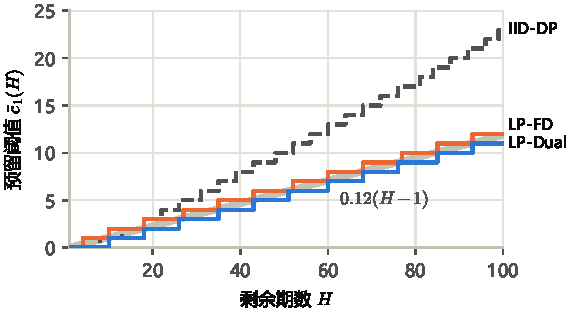
\includegraphics[width=0.64\linewidth]{figures/threshold.pdf}
\caption{预留阈值 $\bar c_1(H)$：库存不超过该值时，类型 1 顾客不再看到商品 1（$c_2=35$，$c_3=25$）。灰线为类型 2 对商品 1 的流体需求 $0.12(H-1)$}
\label{fig:threshold}
\end{figure}

\LPFD{} 的阈值更高，原因在于有限差分在销售期末尾高估最后几件库存的价值。取 $c_1=1$，商品 2、3 充裕，剩余 $\tau$ 期内商品 1 的总流体需求为 $(0.5\times0.6+0.3\times0.4)\tau=0.42\tau$，其中类型 2 的需求为 $0.12\tau$。当 $3\le\tau\le8$ 时 $0.12\tau<1<0.42\tau$，$F(\tau\lambda,\cdot)$ 关于 $c_1$ 在 $[0,0.12\tau]$ 上的斜率为 10（每件都能卖给没有替代选择的类型 2），在 $[0.12\tau,\,1]$ 上的斜率为 9，于是
\begin{equation}
\beta_1=9,\qquad \Delta_1=10\times0.12\tau+9\times(1-0.12\tau)=9+0.12\tau>\beta_1.
\label{eq:fdend}
\end{equation}
类型 1 顾客的商品 1 评分 $0.6(1-0.12\tau)$ 低于商品 3 的 $0.6$，\LPFD{} 不再向类型 1 推荐最后一件商品 1；\LPDual{} 的两件商品评分相等，按即时收益推荐商品 1。真实情况是，剩余 $\tau$ 期内出现一位想买商品 1 的类型 2 顾客的概率为 $1-0.88^{\tau}$，$\tau=5$ 时只有 $47\%$。\LPFD{} 为它保留的最后一件商品 1 常常到期末仍未售出。（$\tau\le2$ 时总流体需求 $0.42\tau<1$，商品 1 不再稀缺，$\beta_1=0$，而 $\Delta_1=3.9\tau$ 仍为正数，\LPFD{} 同样偏保守。）第\ref{sec:where}节用精确的损失分解验证这一机制。
